\chapter{Physical Properties of Low Temperature RF Plasma}
%
	In this first chapter I will provide the necessary physical background for this work about the numerical simulation of low temperature capacitively coupled radio frequency plasma. Here both the mathematical basics and method for the simulation, as well as the most important aspects about the plasma properties will be explained.
%
	\section{Plasma Physics}\label{sec:plasmaphysics}
%
  	\subsection{Capacitively Coupled Radio Frequency Plasma}\label{sec:ccrf}
%
		The experiment where after the conducted simulations is modelled after revolves around a capacitively coupled radio frequency, low temperature plasma at low pressures of oxygen. Here, I will refer to a plasma as an globally quasi-neutral gas, consisting of freely moving charges --- e.g.\@ electrons, positiviely and negatively ions --- and neutral gas particles. The ratio between charged and neutral species defines the \emph{degree of ionization}, which in this case is very low. The term of global neutrality emphasizes the purpose for different lenght scales inside the gas itself. Hence, the associated condition of neutrality by equal densities $n\ix{e}\,=\,n\ix{i}$ only is valid for areas larger than the so called \emph{Debye sphere}. Inside this ball with a radius of $\lambda\ix{D}$ the \emph{Debye length}, the afore-mentioned neutrality is not satisfied.\\
		The creation of a plasma is accomplished by 2 parallel metal plates, the electrodes, where on at least one an ac signal at radio frequency is applied --- this kind of experimental setup is among the most common, thus being used for basic but also in-depth studies of the afore-mentioned discharges. Here, a rf signal at exactly $\unit[13,56]{MHz}$ with an amplitude between $100$--$\unit[1000]{V}$ will be used. This equals to a wavelength of $\unit[22,11]{m}$ for the electric field wave, which is orders of magnitude higher than the eventually simulated experiment. The use of external magnetic fields is not within the scope of this work --- correspondingly, the experiment I will refer to, also did not include any kinds of magnetic confinement or manipulation. \\
			That said, a multitude of electric setups are possible, such as coated or grounded electrodes. Therefore, different regimes of operation ensue. For example, differently driven or shaped metal plates heavily influence the charge creation process inside the plasma. In summary, the electrodes, neutral gas and electric layout resemble a dielectric hindered plate capacitor.
%
		\begin{wrapfigure}{r}{0.42\textwidth}
			\centering
			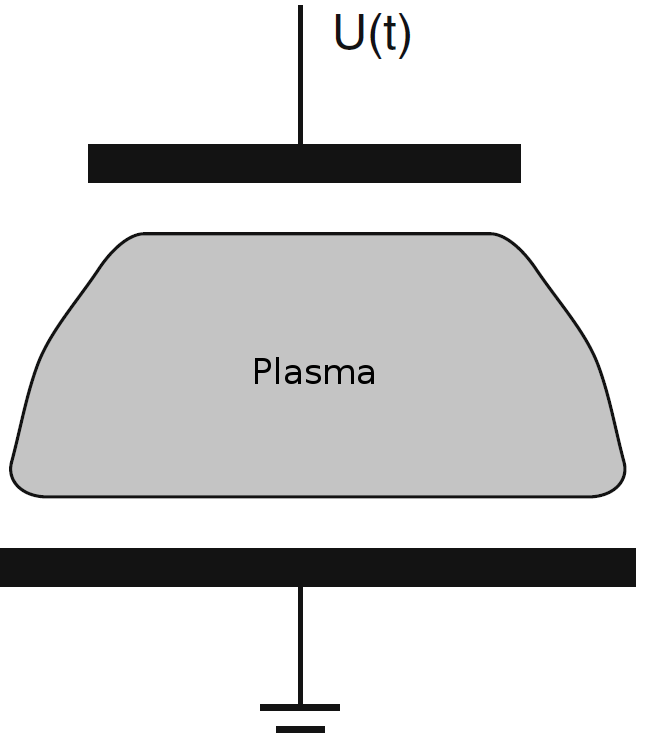
\includegraphics[width=0.38\textwidth]{figures/circuitselfbias_1.png}
			\caption{%
				Schematic of an asymmetric discharge with one grounded and one driven electrode.%
				The rf signal is denoted with $U(t)$.}\label{fig:circuitselfbias_1}
		\end{wrapfigure}
%
		This simplification can be used to access important physical properties, such as an additional voltage offset on one of the electrodes or charge currents at such. A basic scheme of an asymmetric rf discharge can be seen in~\autoref{fig:circuitselfbias_1}. In the case of different electrode sizes, as seen in the scheme, the potential inside the spatially restricted area between wall and discharge can change drastically. This plasma sheath forms also between grounded parts of discharge containment or probes and plasma volume. This additional direct current offset is called \emph{self-bias} (see~\autoref{sec:selfbias}). A dielectric displacement current between plasma sheath and volume accomodates as a result of the different time scales of particle movement (see~\autoref{sec:displacementcurrent}). Especially, self-bias and displacement current play a key role in the following investigations, as a capacitive coupling between electrodes and power supply is difficult to model in a numerical kinetic simulation.\\
		A strong mathematical analysis of general plasma properties would not be suitable for this kind of work, although certain aspects will be discussed later, such as in~\autoref{sec:selfbias} and~\autoref{sec:displacementcurrent}.
		In comparison to other low temperature, low pressure discharges  --- an example could be a dielectric hindered dc discharge at high voltages, with an electrode space gap of just a couple millimeters ---, radio frequency plasma are characterized by their unique transport process inside the sheath and heating mechanisms of charged species. A more in-depth discussion can be found in~\autoref{sec:heating}.\\ 
%
		\subsection{Sheath Physics and Wall Interaction}\label{sec:sheathphysics}
%
			In the discharges bulk, neutral gas particles are exctited by electron collisions and radiating visible light. However, areas around, e.g.\@ floating metal surfaces, probes and grounded walls are darker than the bulk. This is due to the low electron density and kinetic energy in this \emph{plasma sheath}. Though areas with vanishing electron numbers can glow because of high collision efficiencies and/or frequencies.\\
			Electrons, in general, are of a much higher mobility $\mu\ix{e}$ and thermal velocity $v\ix{th,e}$. Hence they impinge onto walls and surfaces more often than other species, leading to a --- in this case we consider an electronegative oxygen discharge, where the following can be assumed true --- negative charge and potential.
%
			\subsubsection{Child-Langmuir Law}\label{sec:langmuirlaw}
%
				For an asymmetric ccrf discharge, dc \emph{self bias} and displacement current are important parts of the electric system. Hence, the \emph{Child-Langmuir Law} as a function of those properties can be written. The rf component of the excitation is neglected.\\
				A greatly negative charged wall at $x=0$ shall be a barrier for electrons of thermal velocity, e.g.\@ $|\Phi(0)-\Phi(d)|\ll k\ix{B}T\ix{e}/e\,$. The thickness of the sheath shall be considered $d$. In an one-dimensional approach, the electron density $n\ix{e}(x)$ can be written with a \emph{Boltzmann} distribution function $f\ix{B}(\Phi)$:
%
				\begin{align}
					n\ix{e}(x)=n\ix{e}(d)\cdot f\ix{B}(\Phi)=%
					n\ix{e}(d)\cdot%
					\exp{\left(\frac{e{\left(\Phi(x)-%
							\Phi(d)\right)}}{k\ix{B}T\ix{e}}\right)}\quad.%
					\label{equ:electrondens}
				\end{align}
%
				This means that the electron density decreases exponentially towards the negatively charged wall. It can be assumed that the sheath thickness $d\ll s\ix{mfp,i}$ the mean free path of the ions inside the plasma bulk. Hence, ions enter the sheath collisionless.\\
				At the boundary between bulk and pre-sheath, the walls potential vanishes because of the plasmas shielding capabilities. Here, the ions are at $v\ix{i,0}$ speeds, therefore their density becomes:
%
				\begin{align}
					n\ix{i}(x)=n\ix{i}(d){\left(1-\frac{2e\Phi(x)%
							}{m\ix{i}v\ix{i,0}^{2}}\right)}^{-1/2}%
					\label{equ:iondens}
				\end{align}
%
				Futhermore, one can assume that the kinetic energy at this point is smaller than the potential energy for the acceleration inside the pre-sheath, e.g.\@ $m\ix{i}v\ix{i,0}^{2}\ll |e\Phi(x)|$. Using \emph{Poisson's } equation, and taking into account the ion-sheath interaction,~\autoref{equ:phibypoisson} gives an equation for $\Phi(x)$:
%
				\begin{align}
					\Delta\Phi\cong-\frac{en\ix{i}{\left(-d\right)}%
							}{\varepsilon\ix{0}}{\left(-\frac{2e\Phi{%
							\left(x\right)}}{m\ix{i}v\ix{i,0}^2}\right)}^{-\frac{1}{2}}%
					\label{equ:phibypoisson}
				\end{align}
%
				Solving this, and using the unpertubated ion current $j\ix{i}=n\ix{i}(d)ev\ix{i,0}$, one yields the result by \emph{Langmuir}.
%
				\begin{align}
					\Phi{\left(x\right)}={\left({\left(\frac{3}{4}{\left(x+d%
							\right)}\right)}^4{\left(\frac{j\ix{i}}{\varepsilon\ix{0}%
							}\right)}^2\frac{m\ix{i}}{2e}\right)}^{\frac{1}{3}}%
					\label{equ:langmuirpot}
				\end{align}
%
				Again, solving~\autoref{equ:langmuirpot} for the current $j\ix{i}$ yields the \emph{Child-Langmuir Law} (see~\autoref{equ:childlangmuirlaw}).\\
				This equation defines the ion current as a function of the unpertubated plasma bulk. In other words, the sheath changes its thickness in dependency of those certain discharge parameters, always satisfying the ion current defined by the \emph{Child-Langmuir Law}.
%
				\begin{align}
					j\ix{i}=\frac{4}{9}\varepsilon\ix{0}{\left(\frac{2e{%
							\left(\Phi{\left(-d\right)}-\Phi{\left(0\right)}%
							\right)}^3}{m\ix{i}d^2}\right)}^{\frac{1}{2}}%
					\label{equ:childlangmuirlaw}
				\end{align}
%
			\subsubsection{Surface Effects and Secondary Ion Emission}\label{sec:surfaceeffects}
%
				Although plasma sheath physics are influenced by bulk properties, such as temperatures and densities, the space charge area itself is mainly characterized by processes of the wall. Hence an important aspect is the absorption and re-emission of ions and electrons.	Those species than have unique features, like e.g.\@ high velocities. Let's assume the associated metal wall behind the sheath ideally absorbs all impinging, charged particles, which recombinate immediately near the surface.\\
%
				\paragraph{Secondary Electron Emission}
				The discharges electrons are much faster and mobile than the other species, leading to the afore-mentioned negative charging and potential drop towards the wall. This accelerates the ion species up to \emph{Bohm velocity} --- see~\autoref{sec:bohmcriteria} for a more in-depth discussion of the \emph{Bohm criteria} and the ions sheath physics.\\
				Continuity and charge conservation must be satisfied, hence the fluxes $J\ix{j}$ of the species $j$ must be equal at the sheath edge --- into and out of the sheath:
%
				\begin{align}
					J\ix{e}=J\ix{i}%
					\label{equ:sheathequi}
				\end{align}
%
				The mentioned potential drop $\Delta\Phi$ from~\autoref{sec:langmuirlaw}, beside accelerating positive ions, reflects negative charges slower than $v\le \sqrt{2e\Delta\Phi/ m}\,$. Similar to~\autoref{equ:electrondens}, the electron current towards the wall can be written. Here the first moment of the electron velocity $\bra v\kett$ is used, calculated in~\autoref{equ:firstmoment} with the electron energy distribution function (EEDF) $f\ix{e}(v)$:
%
				\begin{align}
					j\ix{e}=&-\frac{e}{4}n\ix{e}\bra v\kett\exp\left(-\frac{e\Delta\Phi}{k\ix{B}T\ix{e}}\right)%
					\label{equ:electroncurrent}\\[0.0cm]
					\bra v\kett=&\int_{\mathbb{R}}v\cdot f\ix{e}\left(v\right)\diff v%
					\label{equ:firstmoment}
				\end{align}
%
				Impinging ions are neutralized before impact by particles from the electron gas in the wall. Like before, any produced neutrals are reflected and exit the sheath collisionless --- the mean free path is larger than the sheath thickness. Hence ionization is a process almost exclusively happening in the bulk or the pre-sheath.\\
				Assuming a fast electron impacts on the wall, there is a chance of colliding with and liberating a second electron from the target. Here, the \emph{secondary electron emission} coefficient is noted as $\gamma$: an impinging electron emits $\gamma$-many electrons from the metal. This \emph{SEE} reduces the $\Delta\Phi$ because of an addition charge current from the wall towards the sheath edge, therefore altering the continuity condition $j\ix{i}=j\ix{e}$. A new \emph{effective potential drop} $\Delta\Phi\ix{eff}$ can be written in~\autoref{equ:effectivepotentialdrop}. According to~\cite{} there is a critical value $\gamma\ix{c}$ from which on the wall potential is unstable, leading to shifting sheath edges --- the sheath edge oscillates with the rf signal anyway --- and strong currents from the wall.
%
				\begin{align}
					\Delta\Phi\ix{eff}=-\frac{k\ix{B}T\ix{e}}{e}\cdot\ln\left(\left(1-%
							\gamma\right)\sqrt{\frac{m\ix{i}}{2\pi m\ix{e}}}\,\right)%
					\label{equ:effectivepotentialdrop}
				\end{align}
%
				\paragraph{Secondary Ion Emission}	
				Research~\cite{Kuellig&Meichsner} prior to this thesis indicates that ions are produced near the surface of a metal electrode and heavily accelerated in the plasma sheath. In theory, secondary emission by surface ionization --- in analogy to the surface neutralization --- occurs with incident atoms of thermal energy. Hence one assumes a positively biased wall at high tempertures as the target. It's valence level is therefore broadened, giving an atom $A$ the chance the deposit an electron at the metal. After equilibriating thermally, a positive ion is emited by chance. This statistical process can be described by an thermodynamical equation (see~\autoref{equ:postiveion}) yielding the ionization coefficient of $A$. In~\autoref{equ:sahalangmuir} a modified approach for the \emph{Saha-Langmuir equation} on the degree of ionization in gases can be found. Here, the surface's temperature $T$ and average work function $\overline{\Phi}_{+}$ are needed. Additionally, the ionization energy $I(A)$ --- or impact energy ---, the particle number currents of both species $j$ and $j^{+}$, corresponding statistical weights $w$, $w^{+}$ and reflection coefficients at the intrinsic potential barrier $r$/$r^{r}$ are used.
%
				\begin{align}
					A\leftrightharpoons A^{+}+&\,e^{-}%
					\label{equ:positiveion}\\[0.0cm]
					\alpha^{+}(A^{+})=\frac{j^{+}}{j}=\frac{(1-r^{+})\,w^{+}}{(1-r)\,w}\cdot&\exp\left(%
					\frac{\overline{\Phi}_{+}+e\sqrt{eV\ix{ext}}-I(A)}{k\ix{B}T}\right)%
					\label{equ:sahalangmuirpos}
				\end{align}
%
				At high temperatures of, e.g.\@ $\unit[1000]{K}$ and externally applied potentials $V\ix{ext}<\unit[1]{kV}$, the reflection associated \emph{Schottky term} $e\sqrt{eV\ix{ext}}$ and the corresponding coefficients $r$/$r^{+}$ can be neglected --- it appears to be just half of the thermal energy at room temperature. Though a theoretical approach is possible, there have'nt been accurate studies of such coefficients for temperatures around $\unit[300]{K}$.\\
				In addition to SIE of positive ions, a case for negative ions can be easily derived with small changes to~\autoref{equ:sahalangmuirpos}: a negatively biased electrode is assumed and the average work function yields a different sign. The electron affinity of the incident particle $B$ is noted as $A(B)$.
%
				\begin{align}
					B+\,&e^{-}\leftrightharpoons B^{-}%
					\label{equ:positiveion}\\[0.2cm]
					\alpha^{-}(B^{-})=\frac{(1-r^{-})%
						\,w^{-}}{(1-r)\,w}\cdot&\exp\left(%
						\frac{-\overline{\Phi}_{-}+e\sqrt{eV\ix{ext}}+A(B)}{k\ix{B}T}\right)%
					\label{equ:sahalangmuirneg}
				\end{align}
%
				Applying the former assumptions to both equations of positive and negative ions, inserting a homgeneous work function $\Phi=\overline{\Phi}_{-}=\overline{\Phi}\ix{+}$ for the used substrate yields the originally derived \emph{Saha-Langmuir equations}.
%				
				\begin{align}
					\alpha^{+}(A^{+})=\frac{w^{+}}{w}\,\exp\left(\frac{%
						\Phi-I(A)}{k\ix{B}T}\right)\,\,,%
						\quad\quad%
					\alpha^{-}(B^{-})=\frac{w^{-}}{w}\,\exp\left(\frac{%
						-\Phi+A(B)}{k\ix{B}T}\right)%
						\label{equ:sahalangmuirshort}
				\end{align}
%
				Though only considering atomic particle beams onto the wall until this point, forms similar to~\autoref{equ:sahalangmuirshort} can be derived for molecular surface interactions. In case of the earlier discussed ccrf discharges, arguments like high temperatures can not be applied, hence the need for measured reflection coefficients.\\
				Works of, e.g.\@~\cite{Ustaze97} and~\cite{Los90} investigated ion beam scattering, electron loss and transport in plasma sheath enviroments for metal walls, especially $\text{MgO}(100)$ surfaces. There Ustaze et al.\ studied incident oxygen gas particles --- ions and neutrals ---  on magnesium oxyde surfaces. Impinging atoms became negatively charged ions, picking up electrons from the $\text{MgO}$ of the wall. This interaction, though requiring a minimum ionization and liberation energy for the electron, is most effective at low energies $<\unit[1]{eV}\,$. This is due to a maximum of residence time at the target for an incoming atom. Hence it can be considered a non-resonant charge transfer process at the anion site. For an more in-depth discussion of both electron loss and capture for anion transport processes at walls one should consider~\cite{Kawano83}.\\
				
%
		\subsection{Bohm Criteria}\label{sec:bohmcriteria}
%
			In~\autoref{sec:sheathphysics} the behaviour of charge particle densities inside the plasma sheath has been discussed. In contrast to the discharge volume, those densities do not satisfy the quasi-neutrality condition in a distance of $d$ from the wall anymore. Though we know that the sheath is a spacially restricted area around electrostatic floating surfaces, a physical law concerning this circumstance has not been derived here. So the question ensues, why the area of electron depletion does not extend further into the discharge volume.\\
		To answer this question, one has to take a look at a substitutional system. This will be a, likewise mechanical, one-body extremal problem of a point mass. In this case only kinematic pontentials with inverted parabolic maxima are of interest. Therefore, in this unstable equilibrium, a small pertubation culminates into a large force on the test body.\\
		To see the quality of this example, one has to take a look at the second order differential equation of the afore-mentioned mechanical problem and the electrostatic \emph{Poisson's equation} (see~\autoref{equ:pseudo}).
%
  	\begin{align} 
  	  m\frac{\diff^{2}\vec{r}}{\diff t^{2}}=-\frac{\diff V}{\diff\vec{r}}%
					\quad\Leftrightarrow\quad%
					\Delta_{\vec{r}}\Phi=-\frac{\diff\Psi}{\diff\Phi}=f{\left(\Phi\right)}%
					\hspace{-0.33cm}\overset{\text{Poisson's}}{\overset{\mid}{=}}\hspace{-0.33cm}%
					\frac{\rho}{\varepsilon\ix{0}}%
			\label{equ:pseudo}
  	\end{align}
%
		\begin{figure}[!t]
			\centering%
			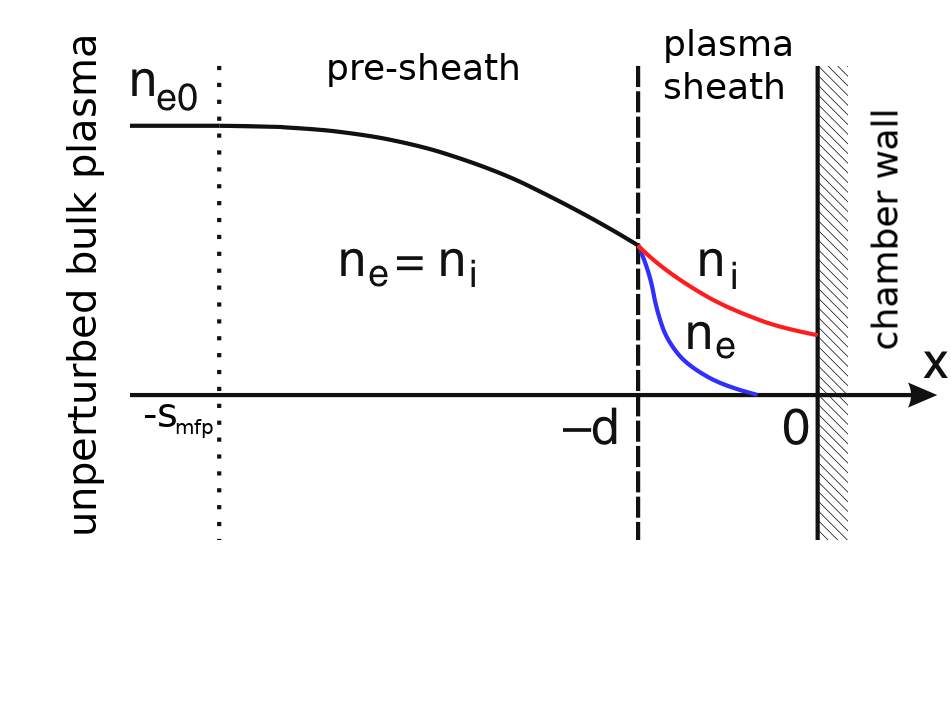
\includegraphics[width=0.6\textwidth]{figures/sheath_piel.png}%
			\caption{%
			One dimensional density profiles as a function of the distance to a floating wall. Note the exponential decrease of the electron density $n\ix{e}$ from the sheath border towards the presumably negatively charged wall. Densities allready reach approximately $0,66n\ix{e,0}$ inside the pre-sheath.}\label{fig:sheath_piel}
		\end{figure}
%
		For an instability, the force on the test body must increase with the distance from the equilibrium, hence the~\autoref{equ:inequality} is used to calculate the exact velocity at which an ion is entering the sheath. This results in the first \emph{Bohm criteria}.
%
		\begin{align}
			0>\left.\frac{\diff^{2}\Psi}{\diff\Phi^{2}}\right|_{\Phi=0}%
			\overset{\text{\autoref{equ:pseudo}}}{\overset{\mid}{=}}%
					\left.\frac{\diff}{\diff\Phi}\left(\frac{n\ix{e}\left(x\right)-n\ix{i}%
					\left(x\right)}{\varepsilon\ix{0}}\right)\right|_{\Phi=0}&%
					\frac{en\ix{e}\left(-d\right)}{\varepsilon\ix{0}}\left(\frac{e}%
					{k\ix{b}T\ix{e}}-\frac{e}{m\ix{i}v\ix{i,0}^{2}}\right)%
			\label{equ:condition}\\[10pt]%
			\Rightarrow\quad%
			v\ix{i,0}\ge v\ix{i,B}=\sqrt{\frac{k\ix{B}T\ix{e}}{m\ix{i}}}&%
			\label{equ:inequality}
		\end{align}
%	
		Analoguos you can define the so called \emph{Mach number} $M=v\ix{i,0}/v\ix{i,B}$, where $v\ix{i,B}$ denotes the \emph{Bohm velocity}.\\
		Now, to understand why the sheath does not extend further than a fixed distance $d$ from the discharge boundary, the particle movement has to be investigated on a smaller scale. As seen above, there is an electric field in the \emph{pre-sheath} that accelerates the ions to $v\ix{i,B}$. In addition, quasi-neutrality is still satisfied here:
%
		\begin{align}
			n\ix{i}\left(x\right)=n\ix{i,0}\exp\left(\frac{e\Phi\left(x\right)}{k\ix{B}T\ix{e}}\right)%
			=n\ix{e}\left(x\right)\,\,.%
			\label{equ:quasineutral}
		\end{align}
%
		Still, $\Phi{\left(x\right)}$ is the potential inside the pre-sheath from~\autoref{sec:sheathphysics} and $n\ix{i,0}$ the unpertubated density from the plasma \emph{bulk}. A greater part of the ion transport process in this area is governed by collisions with neutral gas particles, hence the velocity distribution function with the collision frequency $\nu\ix{n,i}$ has to be rewritten:
%
		\begin{align}
			\frac{\diff v\ix{i}}{\diff x}=\frac{\nu\ix{n,i}v\ix{i}^{2}}{v\ix{B}^{2}-v\ix{i}^{2}}\quad.%
      \label{equ:distribution}
		\end{align}
%
		From the singularity in~\autoref{equ:distribution} at $v\ix{i}=v\ix{B}$ and the knowledge of $\Phi(x)$ at the wall, one can calculate the sheath thickness $d$. Furthermore, ions with velocities smaller than the Bohm velocity are being accelerated inside the pre sheath. According to~\autoref{equ:inequality} velocities greater than $v\ix{B}$ are not allowed here. This is, together with~\autoref{equ:distribution} the reason why the ion velocity is exactly $v\ix{B}$ at the boundary of the plasma sheath and thus a positive space-charge ensues.
%
		\begin{align}
			M\ge1%
			\Leftrightarrow%
			v\ix{i}(-d)\ge v\ix{B}%
			\label{equ:bohmcriteria2}
		\end{align}
%
		Conclusively, at the sheath boundary~\autoref{equ:bohmcriteria2} is satisfied.\\
  At $x=-d$, both negative and positive charge density decreased to $n\ix{i}=n\ix{e}\approx0,66n\ix{e,0}$ (see~\autoref{fig:densities}), where the potential is approximately $-k\ix{B}T\ix{e}/2e$ because of the currents onto the wall.\\
		In summerization, the plasma does not `see' its sheath, because the ion dynamic discussed before is spatially restricted. The sheath only develops where there is electron depletion or an externally applied, negative potential.
%
		\subsection{Self Bias Voltage}\label{sec:selfbias}
%
			An important step towards the electric characterization of such ccrf discharges is the development of a replacement circuit, see~\autoref{fig:circuitselfbias_1}. Thus, one can define a specific impedance for a rf discharge of excitation frequency $\omega$. The valeu of $\varepsilon\ix{p}$ resembles the permeability of the working gas between the driven and/or grounded electrode. In addition, this volume has the capacity $C\ix{p}$ --- the capacity of a cubicle with a cross section $A$, thickness $b$ and electron-neutral collision frequency $\nu\ix{e,n}$ calculates like~\autoref{equ:capacityandepsilon}.
%
			\begin{align}
				\varepsilon\ix{p}=1-&\frac{\omega\ix{p,e}^2}{\omega\left(\omega-\imag\nu\ix{e,n}\right)}\quad\quad%
				C\ix{p}=\varepsilon\ix{p}C\ix{0}=%
				\varepsilon\ix{p}\varepsilon\ix{0}\frac{A}{b}%
				\label{equ:capacityandepsilon}\\[10pt]
				&Z\ix{p}={\left(\imag\omega C\ix{p}+ \frac{1}{\frac{1}{\omega\ix{p,e}^2C\ix{0}}%
						{\left(\nu\ix{e,n}+\imag\omega\right)}}\right)}^{-1}%
				\label{equ:bulkimpedanz}
			\end{align}
%		
			\begin{figure}[!b]
				\centering
				\begin{subfigure}[b]{0.49\textwidth}
					\centering%
					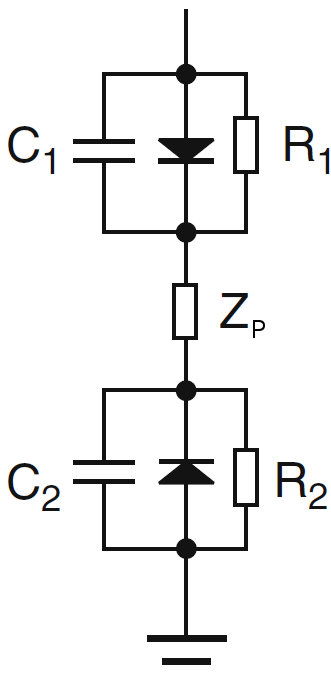
\includegraphics[width=0.4\textwidth]{figures/circuit_selfbias_piel.png}
					\caption{Replacement Circuit}%
					\label{fig:circuitselfbias_1}
				\end{subfigure}
				\begin{subfigure}[b]{0.49\textwidth}
					\centering%
					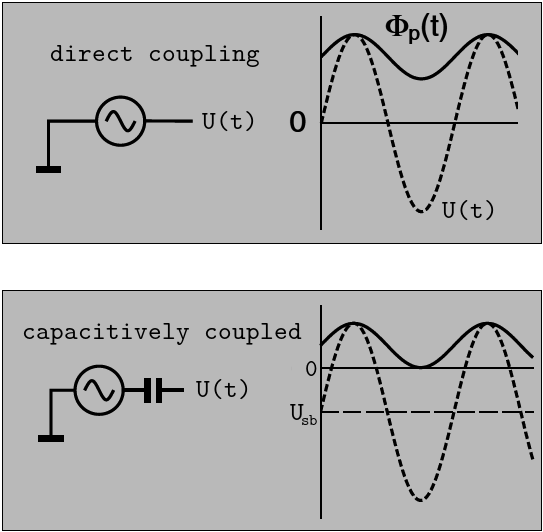
\includegraphics[width=0.8\textwidth]{figures/selfbiasvoltage.png}
					\caption{Voltage and Potential}%
					\label{fig:circuitselfbias_2}
				\end{subfigure}
					\caption{%
					Figure for an asymmetrically driven ccrf discharge.\\%
					(A): $Z\ix{p}$ denotes the impedance of the plasma bulk. A diode represents the directed electron current from the sheath into the discharge volume. $R\ix{j}$ and $C\ix{j}$ are the electrical properties of the positive space-charge area.\\%
				(B): Schematic of potential and voltage of a direct capacitively coupled rf disharge.}%
			\end{figure}
%
      The~\autoref{equ:bulkimpedanz} represents the full electrical impedance, consisting of the inverse sum of real and imagninary resitance, as well as the capacity of the neutral gas volume. Here, $\imag\omega/(\omega\ix{p,e}^{2}C\ix{0})$ characterizes the electrons interia in regard to an external excitation $\omega$. The real part $\nu\ix{e,n}/(\omega\ix{p,e}^{2}C\ix{0})$ denotes the resistance by neutral particle collisions.\\
        For high excitation frequencies, e.g.\@ $\unit[13,56]{MHz}$ the bulk impedance can be neglected. Both sheath capacities of anode and cathode take the dominant part. Therefore, the discharge potential and voltage can be written as:
%
			\begin{align}
				U\left(t\right)=U\ix{sb}+U\ix{rf}\sin\left(\omega t\right)%
        \quad\quad%
        \Phi\ix{p}\left(t\right)=\overline{\Phi\ix{p}}+%
          \Phi\ix{rf}\sin\left(\omega t\right)%
        \label{equ:selfbias_1}
			\end{align}
%
      Both electrodes sheath collapses completely during a full cycle of $U\ix{rf}(t)$, which is why charges can impinge onto the surface and force the plasma potential $\Phi\ix{P}$ to equal out locally with the walls. A short circuit between plasma and sheath occurs when $\Phi\ix{P}$ becomes negative with regard to the excitation. The~\autoref{equ:selfbias_unequal} and~\autoref{fig:selfbias} express this circumstance.
%
      \begin{align}
        \Phi\ix{p}\max=\overline{\Phi\ix{p}}+\Phi\ix{rf}\geq U\ix{sb}+U\ix{rf}%
        \quad\quad %
        \Phi\ix{p}\min=\overline{\Phi\ix{p}}-\Phi\ix{rf}\geq0%
        \,\,.%
        \label{equ:selfbias_unequal}
      \end{align}
%     
      If there is no special coupling between electrode and electrical driver, the equality in~\autoref{equ:selfbias_unequal} is true. However, if a capacitive coupling is used, there can't be any net current between excitation and electrode. The capacitance can not be inverted over the course of one rf cycle. The electron currents are then equal on both electrodes, therefore shifting the minimum plasma potential to ground and the maximum to the excitation.\\
      Finally, the dc \emph{self bias} part $U\ix{sb}$ and the mean plasma potential $\overline{\Phi\ix{p}}$ are
%
      \begin{align}
        \overline{\Phi\ix{p}}=\frac{1}{2}\left(U\ix{sb}+U\ix{rf}\right)%
        \quad\quad%
        U\ix{sb}=\frac{C\ix{1}-C\ix{2}}{C\ix{1}+C\ix{2}}U\ix{rf}%
        \,\,.%
        \label{eq:selfbiaszwei} 
      \end{align}
%     
      If the excitation frequency $\omega$ is small compared to other time scales, e.g\@ electron and ion plasma frequencies, the electron current from the sheath $j\ix{L}$ becomes bigger than the displacement current $j\ix{dc}$. Hence the electron current onto the driven electrode decreases by a maxwellian factor --- this is a function of the thereon apllied voltage --- compared to the corresponding ion current.\\
      Conclusively, the electrodes sheath impedance is bigger than those of the floating walls. Together with~\autoref{equ:selfbias_1} and~\autoref{equ:inequality} the plasma potential $\Phi\ix{p}$ approximately vanishes, requiring only the currents onto the driven electrode to equal out. For small values of $\omega$~\autoref{equ:selfbias_3} yields the \emph{self bias voltage} (~\cite{Piel10}). Here, $\mathbf{J}\ix{0}$ denotes the zeroth order \emph{Bessel function}.
%      
      \begin{align}
        U\ix{sb}=\frac{k\ix{B}T\ix{e}}{e}\ln%
        \left[\mathbf{J}\ix{0}\left(\frac{eU\ix{rf}}{k\ix{B}T\ix{e}}\right)\right]%
        \label{equ:selfbias_3}
      \end{align}
%     
     	In~\autoref{fig:imagandreal} voltage and current are shown for an exemplary ccrf discharge. One can examine there that the self bias never disappears for excitations $U\ix{rf}\neq0$, hence becoming an important part for capacitively coupled plasma.
%
			\newpage
%
    \subsection{Dielectric Displacement Current}\label{sec:displacementcurrent}
%
    	\begin{wrapfigure}{r}{0.47\textwidth}
    	  \centering%
    	  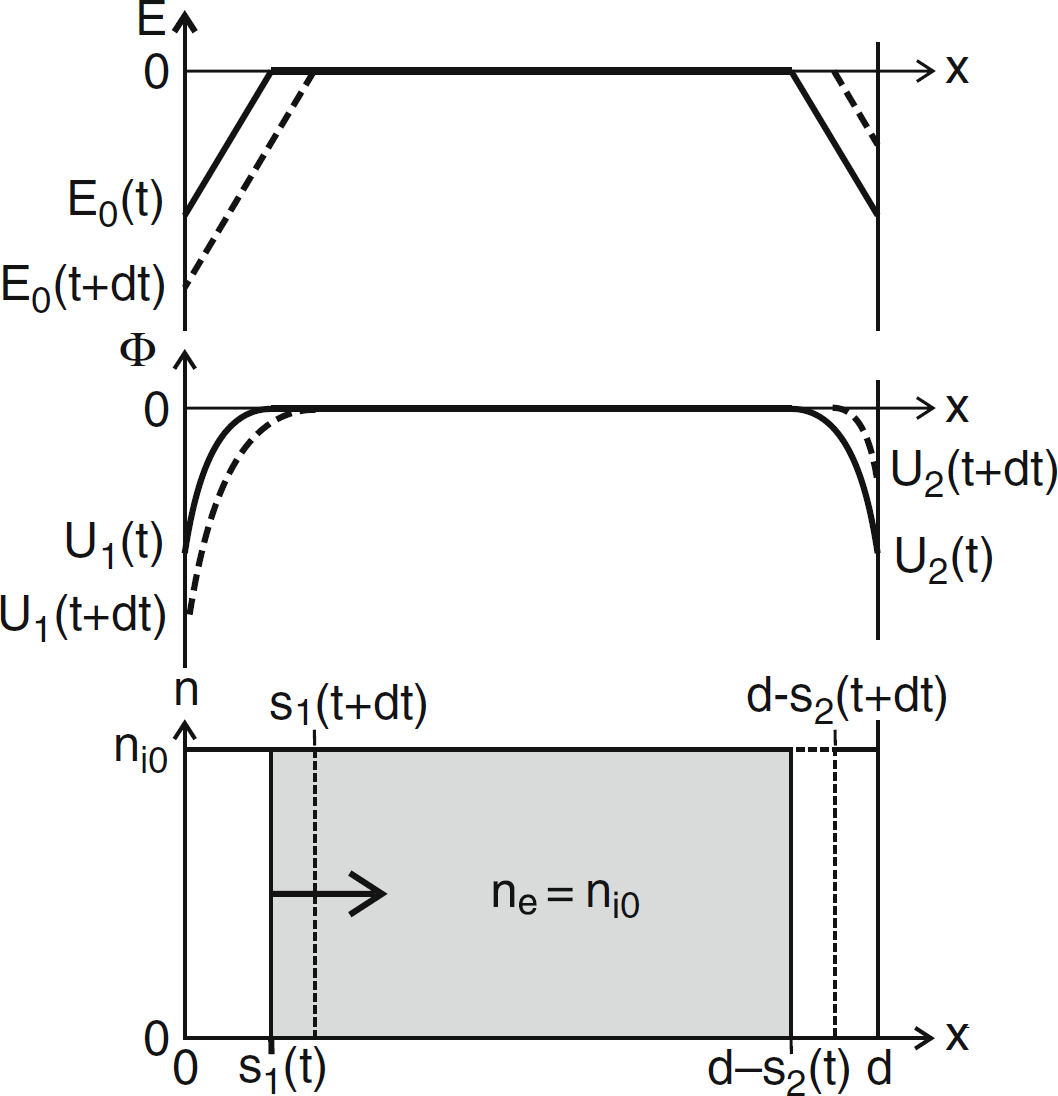
\includegraphics[width=0.45\textwidth]{figures/displacement_current_piel.png}%
    	  \caption{%
    	    One dimensional density, potential and electric field for an asymmetric, harmonically driven discharge. Note the moving sheaths border.}%
					\label{fig:displacementcurrent}
    	\end{wrapfigure}
%
    	Due to their higher mobility and plasma frequency $\omega\ix{p,e}$, the electron distribution can follow an external excitation with a similarly high frequency much better than the heavier ions species. Because of that, one will assume those as nearly stationary, e.g.\@ $\omega\ix{p,i}\ll\omega\ix{p,e},\,\omega\ix{rf}\,$. Investigating the circumstances and consequences of this relation yields the displacement current $j\ix{d}$. \\
    	Lets suppose there is an area of thickness $d$ in front of a negatively charged wall, where the electron density is negligible and the corresponding ion property constant at $n\ix{0,i}$. Thus an electric field of
%   	 
    	\begin{align}
    	  E\ix{0}=-en\ix{0,i}d/\varepsilon\ix{0}
    	\end{align}
%
    	establishes. If the wall potential now decreases due to electron bombardement or external manipulation, the sheaths border moves further inside into the discharges volume with the veloctiy $v=\diff s\ix{1}/\diff t$. Thus, the sheath expansion and hence charge movement creates an additional \emph{displacement current} $j\ix{d}$, which is compensated with $j\ix{d,e}$ the electron current from this border displacement. Hence charge conservation and continuity is satisfied.
%
    	\begin{align}
    	  j\ix{d}=-en\ix{0,i}v=-j\ix{d,e}
    	\end{align}
%
    	Electrons that are puished out of this positive space-charge area then contribute to the plasma bulk density, and conclusively, to the quasi neutrality $n\ix{e}=n\ix{0,i}\,$. But in case of a harmonically driven discharge, the sheath in front of the opposing electrode is shrinking with $\diff s\ix{1}=-\diff s\ix{2}\,$. Hence, the bulks spatial expansion and position are oscillating sinusoidal, or: the sheaths thickness oscillates harmoncally around a mean value, e.g\@ $s\ix{0}$. The associated voltage drop across the discharge between the sheath potentials $U\ix{1/2}$ would be
%
    	\begin{align}
    	  \Delta U=U\ix{1}-U\ix{2}=-\frac{2en\ix{i,0}s\ix{0}}{\varepsilon\ix{0}}\exp{\left(\imag\omega t\right)}
    	\end{align}
%
		\subsection{Heating Mechanisms}\label{sec:heating}
%
  \section{Negative Ion Physics}
%
    \subsection{Anion Creation and Distribution}
%
    \subsection{Dynamics and Collisions}
%
  \section{Particle-in-Cell Cimulations with Monte Carlo-Colissions}
%
    \subsection{Principles}
%
    \subsection{2d3v PIC}
%
    \subsection{Monte Carlo-Collisions}
